\chapter{Design og Implementering}
I dette kapitel vil vi gennemgå forskellige teknologier, der er benyttet i udviklingen af systemet.
Vi vil også redegøre for arkitekturen af systemet, ved brug af et klassediagram og et komponentdiagram, efter UML standarden, til at visualisere og illustrere systemets opbygning.
Den sidste del af kapitlet vil berøre systemets forskellige komponenter og beskrive dem med kodeeksempler og detaljer om implementering af de vigtigste og mest interessante dele. 
Undervejs vil vi, i gennemgangen af komponenterne, konkludere på deres implementering og ikke mindst betydning for systemet, blandt andet i forhold til de user stories, der omhandler den givne komponent.

\section{Anvendte teknologier}
I dette afsnit beskrives teknologierne, gruppen har valgt at anvende til udviklingen af projektet.
Disse teknologier er valgt for at opfylde studieordningen, hvor C\# skulle være det anvendte programmeringssprog, og desuden for at behjælpe i at opfylde kravene stillet i \myref{sec:krav}.

\subsection{Bootstrap}
``Bootstrap'' er navnet på et front-end web udviklings framework, oprindeligt udviklet af Twitter til eget brug, men senere frigivet som open source. 
Bootstrap er i følge dem selv ``[...] the most popular HTML, CSS, and JS framework for developing responsive, mobile first projects on the web.'' \cite{GETBOOTSTRAP}
Som de selv skriver så giver Bootstrap mulighed for at bruge den samme teknologi på tværs af enheder, dette gør det nemmere for udviklere at give brugeren en mere konsistent oplevelse.
Et af de vigtigste koncepter bag Bootstrap er at hver side består af et gitter som er 12 kolonner. 
På den måde er det nemt at bestemme bredden på et givent element, ved at indgrænse det til en del af sidens bredde, dette vil også automatisk forsøge at skalere sig til en mobil enhed. 
Anvendelsen af Bootstrap sker når man påklæder sine HTML elementer med de givne CSS klasser som Bootstrap udgiver. 
Det er herunder muligt at anvende flere klasser på samme element, samt den samme klasse på tværs af forskellige HTML elementer. 
Dette bidrager til at øge konsistensen i layoutet.
JavaScript bruges i Bootstrap til at animere elementer på siden.
 
Dette øger brugerens interaktion, og bringer Bootstraps elementer til live. \cite{GETBOOTSTRAP}

\subsection{ASP.NET MVC 5}
``ASP.NET MVC 5'' er navnet på Microsofts open source implementering af MVC mønstret (beskrevet i \myref{MVC}). 
ASP.NET MVC er baseret på grundtanken om at opdele de forskellige logiske lag i applikationen: Modellen (``business layer''), Viewet (``display layer'') og Controlleren (``input kontrol''). 
Brugen af ASP.NET giver mulighed for at bruge den såkaldte ``Razor syntax'', som er en del af ``ASP.NET Razor view engine''.
Den gør det muligt at anvende C\#-kode (Eller Visual Basic .NET) i front-enden, til at genere dynamiske hjemmesider. 
Disse udtryk evalueres serverside ved runtime, derfor er alle datatyperne dynamiske, og ikke typesikre, det antages altså ved compiletime at alle operationer er mulige på objekter at typen ``dynamic''. \footnote{http://msdn.microsoft.com/en-us/library/dd264736.aspx}

\subsection{Entity Framework}
Entity Framework (``EF'') er et Object-relational mapping (``ORM'') framework til .NET frameworket, udviklet af Microsoft, og er databasen der bruges i projektet. \citep{EF} 
EF er valgt til dels grundet at det er muligt at udvikle ``Code-first'', hvilket vil sige at udvikleren først skriver modellen som klasser, hvorefter databasestrukturen kan opbygges. 
Der understøttes komplicerede relationer såsom mange-til-mange og en-til-mange, ved brug af en relationsdatabase, som er en tabel der kæder 2, eller flere, informationer sammen på tværs af tabeller.

\section{Arkitektur}
Dette afsnit beskriver arkitekturen der benyttes i implementationen for systemet.
Først gennemgås design mønsteret der benyttes, derefter systemets klasser, samt dets komponenter.

Nogle komponenter har vi valgt at benytte, ASP.NETs indbyggede programdele.
Vi benytter os af en færdig login løsning, der er tilgændeligt i ASP.NET teknologien (se eventuelt \myref{apsnet}).
Dette har vi valgt, da vi har vuderet at login ikke er en central problemstilling i forhold til studieordningen og projektets mål.
Dette tillader os at bruge mere tid på andre dele af programmet, som vi finder mere relavante i forhold til de opstillede mål.
Denne implementation er udført for at opfylde user story 10.

\subsection{MVC-mønsteret}\label{MVC}
Et af de standardiserede design mønstre, som bruges af mange udviklere er MVC-mønsteret - som står for \textit{Model-View-Controller}.
MVC-mønsteret har til formål, at dele systemet op i tre komponenter, nemlig \textit{Model}, \textit{View} og \textit{Controller}.
Denne segregering adskiller således ''forretnings-logik'', ''input-logik'' og ''UI-logik'', og gør herved systemet mere fleksibelt, samt fremmer muligheden for at udvikle parallelt på de forskellige komponenter.
Dette kan være nyttigt i udviklingen af systemet, men også efter udgivelsen, idet blandt andet ''UI-logik''kan blive ændret oftere end for eksempel ''forretnings-logik''.
Opdelingen hjælper også til at skabe overblik over koden, og gør det nemmere at udføre tests på systemet. \citep{MVC_Overview}

\begin{wrapfigure}{r}{0.4\textwidth}
	\vspace{-20pt}
	\begin{center}
		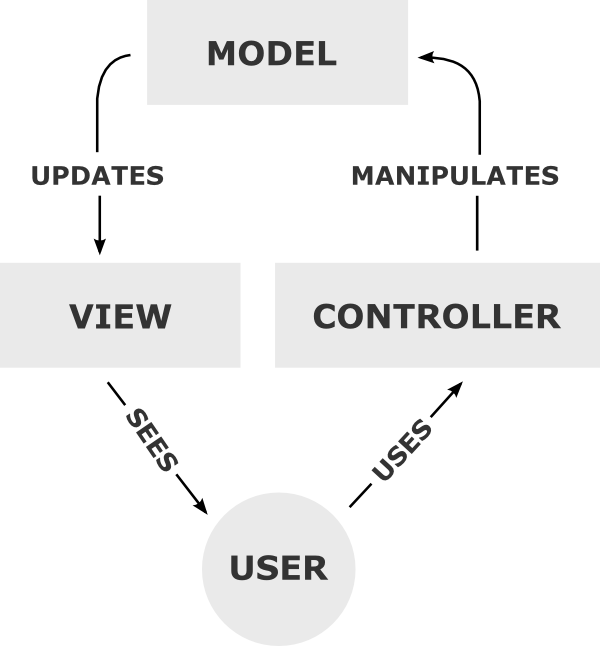
\includegraphics[width=0.38\textwidth]{images/Images/mvc.png}
	\end{center}
	\vspace{-20pt}
	\caption{MVC-mønsteret}
	\vspace{-20pt}
\end{wrapfigure}


Nedenfor beskriver vi de tre komponenter.

\textbf{Model}\\
De objekter, der udgør model-laget skal indeholde den før omtalte ''forretnings-logik'', samt alle data der skal modelleres i systemet.
Dataen, i form af objekter, gemmes oftest i en database eller fil, og er helt skjult for brugeren i den forstand, at al repræsentation af modellen foregår igennem view-delen af MVC-mønsteret.

\textbf{View}\\
Der er igennem forskellige views, at brugeren får præsenteret brugergrænsefladen - også kaldet UI(user-interface).
Derfor giver det også mening, at placere ''UI-logikken'' i denne del af MVC-mønsteret.
Typisk bliver et views indhold genereret ud fra data fra en model.
Et eksempel på dette ville være visning af en liste af objekter ud fra en model, der indeholder netop en liste.

\textbf{Controller}\\
Når det kommer til interaktionen mellem brugeren og systemet, er det controlleren der påtager sig opgaven.
Derfor er det også i de forskellige controllerere, at vi finder ''input-logikken''. Her bestemmes ud fra input fra brugeren hvilke data der skal arbejdes med i hvilken model og også hvilket view, der skal præsenteret for brugeren. Med dette kan vi også se, at viewet ikke indeholder nogenb logik og al manipulation af data altså foregår gennem controller komponenten.


\subsection{Program komponenter}\label{subsec:komp}

Der kan dannes forskellige komponenter i programmet ud fra de user stories der blev opgivet på \myref{sec:krav}.
Disse kan ses på \myref{figure:komp}.
Figuren viser hvordan de forskellige user stories kan deles op i komponenter, og hvordan disse komponenter afhænger og bruger hinanden som beskrevet ud fra vores user stories.

\begin{figure}
	\vspace{-20pt}
	\begin{center}
		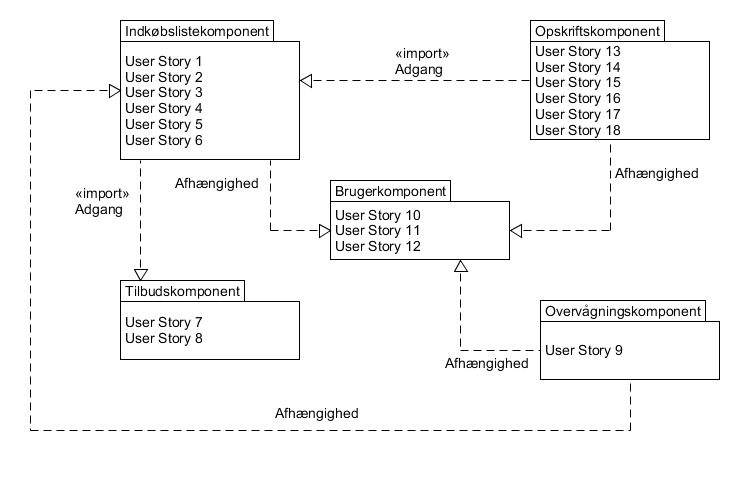
\includegraphics[scale=0.6]{images/Diagrams/Komponenter.png}
	\end{center}
	\vspace{-20pt}
	\caption{UML 2 Komponent diagram }
	\label{figure:komp}
	\vspace{-20pt}
\end{figure}

\textbf{Indkøbslistekomponentet} står for at lave indkøbslister, og tilføje varer og tilbud til disse.
Tilbudene skal importeres fra \textbf{tilbudskomponentet}, for at lave koblingen imellem varerne og tilbud.
Det er afhængigt af \textbf{brugerkomponentet} da indkøbslisterne hører til en bruger for at danne personlige lister. Brugerkomponentet er ansvarlig for alt der har med en bruger at gøre. Det indebærer at registrere hvem der er logget på, håndtere brugerens personlige indstillinger. Det er altså dette komponent der sørger for den personlige oplevelse på hjemmesiden.

\textbf{Opskriftskomponentet} er afhængig af brugerkomponentet, da det er brugerene i systemet der tilføjer opskrifter, samt giver opskrifterne en rating.
Dog er det opskriftskomponentet der står for dette, men det skal dog vide hvem der er logget ind på hjemmesiden.
Der er en adgang her fra til indkøbslisterne for at kunne tilføje ingredienser fra opskrifterne til indkøbslister.

\textbf{Overvågningskomponentet} står for at overvågningen af tilbud for en specifik varer kan foregå.
Der dannes en afhængighed herfra og til indkøbslistekomponentet da overvågningslisten gør brug af de metoder som der stilles til rådighed i dette komponenet, såsom tilføje varer, og finde tilbud.


\subsection{Klassediagram}
For at illustrere modellaget i vores MVC-mønster, har vi produceret et klassediagram (se \myref{diagram:klassediagram} nedenfor) i UML, der simplificerer strukturen.
Det skal bemærkes, at klasserne og felterne er på dansk i diagrammet, og på engelsk i selve koden af programmet. \fxfatal{Der er ingen adgangsting på dette, private, protected, public etc. Er det bevist? Derudover er det ikke klart hvilken datatype hvert felt er, også om det er en liste eller ej. - Troels - Fikser figuren senere - Søren}

\begin{figure}[H]
\centering
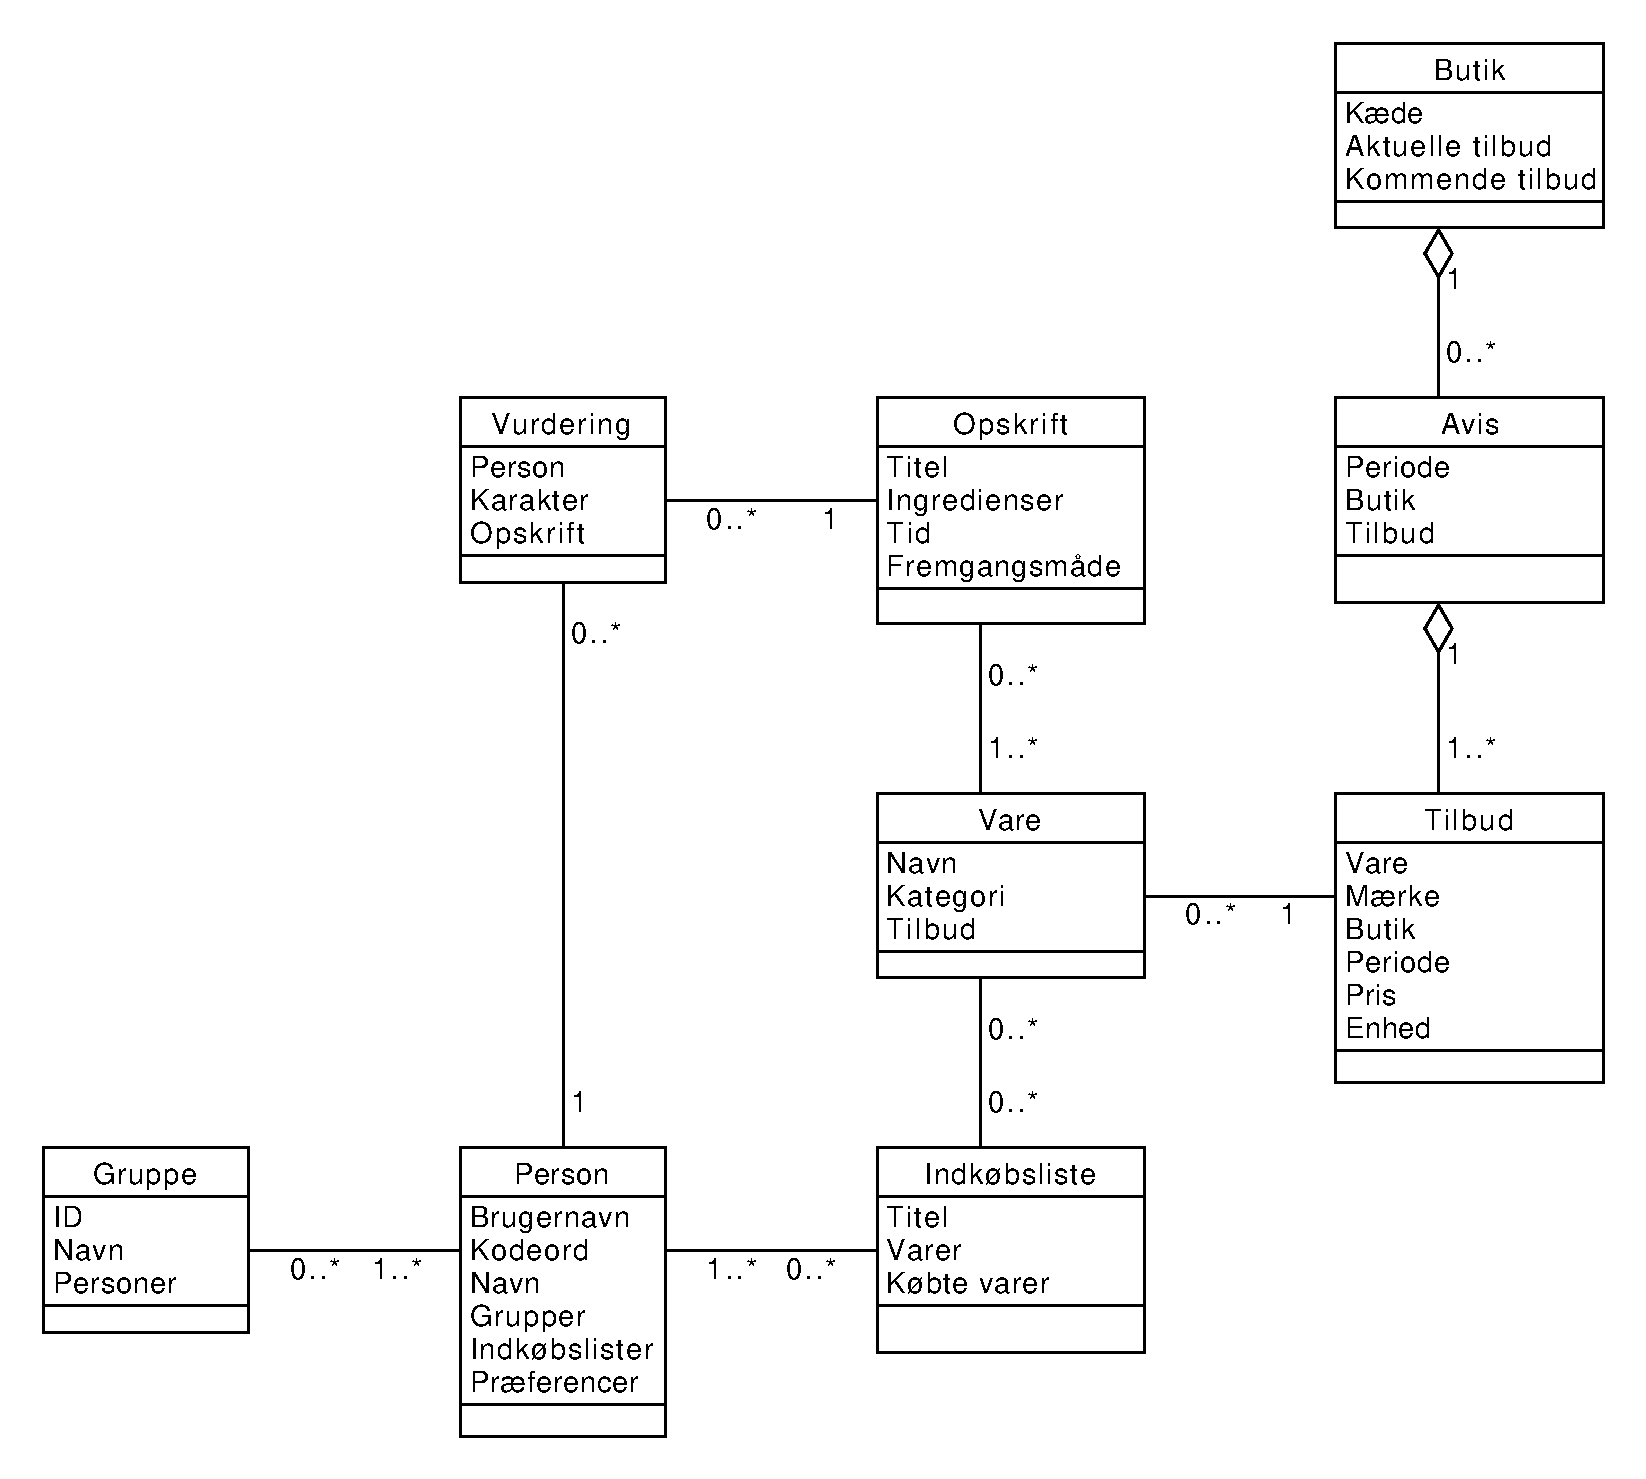
\includegraphics[width=0.8\linewidth]{/Diagrams/klassediagram_model_expanded_implemented.pdf}
\caption{UML klassediagram for modellaget i MVC-mønsteret}\label{diagram:klassediagram}
\end{figure}

\subsection{Klasserne}
Vi vil gennemgå klasserne, der optræder i klassediagrammet, og beskrive deres relationer samt deres felter.

\fxnote{Indsæt figur for hver enkelt klasse.}

\subsubsection{Person}
Person-klassen i modellen, er den der holder styr på brugeren og dennes basale attributter - herunder brugernavn, kodeord og kaldenavn.
Ydermere er det vigtigt, at objektet kan indeholde informationer om personens madpræferencer og vurderinger af opskrifter; dette er med til at give person-klassen en mere intim vinkel, og så at sige bedre afspejle den virkelige person, samt fungere som grundlag for anbefaling af opskrifter.
Det er naturligvis også vigtigt for et program, der omhandler bl.a. indkøbslister, at holde styr på en persons indkøbslister og lignende.
Til dette har person-klassen to felter der hedder henholdsvis, grupper og indkøbslister.
Begge felter er lister\fxfatal{Som nævnt tidligere er dette ikke klart fra diagrammet. - Troels}, der holder styr på personens relationer til netop grupper og indkøbslister - En person kan altså have relationer til flere grupper og flere indkøbslister, hvilket også kan ses ud fra de indtegnede relationer i klassediagrammet.


\subsubsection{Indkøbsliste}
Indkøbslister repræsenteres i systemet som klassen ´´Indkøbsliste'', og indeholder ID, titel og to lister med varer.
ID'et garanterer, at alle indkøbslister er unikke og kan skelnes fra hinanden på systemsiden.
Indkøbsliste-klassen har et titel felt, så brugeren også kan navigere mellem forskellige instanser.
De to lister af varer, holder styr på henholdsvis; varer som bliver tilføjet til listen, og varer som har været tilføjet men er blever markeret som købt.
Der er således kun styr på ''overstregede'' varer - altså dem der er købt, og ikke varer som bliver slettet fra listen.
En indkøbsliste kan godt eksisterer uden varer, idet brugeren skal kunne oprette lister, inden der er taget stilling til, hvilke varer der skal bruges.
Indkøbsliste har kun relation til en gruppe, men kan godt have relationer til flere personer.\fxnote{Findes der stadig to lister - Bruger vi dem ?}

\subsubsection{Vare}
Vare-klassen indeholder tre felter: Et navn på varen, som er generisk, for eksempel ''Letmælk'' og ''Cola'' istedet for ''Arla Letmælk'' og ''Pepsi''; en kategori, der beskriver varen, for eksempel ''Mejeri'' eller ''Pålæg''; og en liste over tilbud, der holder styr på, hvis og hvor varen eventuelt er på tilbud.
En vare behøver ikke være på en indkøbsliste eller opskrift for at eksistere \fixme{kan det passe?}, og kan have relationer til nul til mange tilbud.

\subsubsection{Tilbud}
Et tilbud som instans af Tilbud-klassen, indeholder felter der beskriver: Varen, mærket, hvilken butik tilbuddet befinder sig i, hvilken periode tilbuddet gælder i, prisen på tilbudet, og hvilken enhed/mængde tilbudet er i.
Ud fra disse atributter er det muligt at identificere tilbudet, og brugeren kan tage stilling til, om det er relevant.


\subsubsection{Opskrifter}
\lipsum[1]

\subsubsection{Vurdering}
\lipsum[1]


\newpage
\section{eTilbudsavis API}\label{api}
I dette afsnit beskrives først teori om hvad et API er, og hvordan sådan et er struktureret.
Herefter gennemgås design og implementering for brug af eTilbudsavis' API samt motivationen for at bruge API'en. 
Til sidst vil der blive konkluderet på API'ens betydning for projektet.

User story 7 fortæller at man skal kunne se tilbud.
API'et gør det muligt at indhente infomation om butikker og deres tilbud.
Dette API udbydes af den danske virksomhed eTilbudsavis.dk, og er af typen REST.

\subsection{Teori}
Representational state transfer (REST) er en arkitektur anvendt over HTTP(S) standarden. 
I forbindelse med eTilbudsavisen anvendes der HTTP status koder, som signalerer hvorvidt en given forespørgsel er godkendt, afvist eller lign.

\subsubsection{API-Kald}
For at kommunikere med API'et skal der konstrueres en forespørgsel.
Inden for REST, bruges der de fire mest almindelige HTTP metoder, som er POST, GET, PUT og DELETE.
Disse fire metoder findes tilsvarende i CRUD som: CREATE, READ, UPDATE, DELETE.

\textbf{GET}
returnerer data, typisk som JSON eller XML og med HTTP svarkoden 200 (OK).
eTilbudsavis' API sender JSON.
Svarer til READ i CRUD.

\textbf{POST}
bruges til at oprette nye ressourcer.
Svarer til CREATE i CRUD.

\textbf{PUT}
bruges til at opdatere information, eksempelvis til at forlænge en session.
Svarer til UPDATE i CRUD.

\textbf{DELETE}
bruges til at fjerne ressourcer.
Svarer til DELETE i CRUD.

\subsection{Design}
eTilbudsavis' API er kun et halv-offentligt API, dvs. at man skal have en API-nøgle (``APIKEY'') og dertilhørende hemmelighed (``Secret''), som vi har modtaget eTilbudsavis.
API'en er placeret på \textit{https://api.etilbudsavis.dk/v2/}. \citep{eTilAPI}

For at kommunikere med API'en fra C\#-kode anvendes værktøjet RestSharp. RestSharp er en simpel REST og HTTP API klient for et .NET miljø. \citep{RestSharp}
For at kunne bruge informationen laves der en klasse, som svarer til det JSON som API'en sender tilbage.

\subsection{Vurdering}\label{api:skoddata}
Vi har valgt at benytte et API, især eTilbudsavis' API, da det giver os muligheden for at arbejde med og vise faktiske tilbud.
Der er dog fundet visse ulemper ved, at vi benytter os af eTilbudsavis' API.
Det data, vi modtager, begrænser os fra at udvikle flere funktioner, da det f.eks. ikke indeholder: information omkring mængde tilbud, kategori-inddeling eller forekomster af allergener i varerne. 
Dette er funktioner, vores testpersoner har adspurgt. 
Hvis disse tre attributter havde været tilstede, ville systemet for eksempel være i stand til at frasortere tilbud, der indeholder spor af jordnødder eller lignende, hvis den pågældende bruger eksempelvis er allergisk overfor jordnødder. 
Ligeledes ville det med kategori-inddeling være muligt at sortere mere intuitivt i tilbud, og information om grupperede tilbud ville give systemet mulighed for at præsentere visse tilbud bedre for brugeren, så der ikke opstår forvirring.

\subsection{Implementering}
Denne implementering er en del af controlleren: \class{OfferController.cs}, i metoden \class{ImportOffers}.
\subsubsection{Session}
For at kunne bruge API'et skal man først oprette en session.
En session består af en API-nøgle, den tilsvarende hemmelighed (Secret), en token og en signatur.
Har man en API-nøgle kan man kalde API'et sessions og få en token.
Den token kan man kombinere med sin hemmelighed og generere SHA-256 hashen af dette, som er signaturen, der brugers til at underskrive requests.

Eksempelvis vil API-kaldet, som opretter en session returnere:
\begin{lstlisting}[language=json,firstnumber=1,caption={POST til sessions API'et med APIKEY'en},label=apilst1]
{
    "token": "00hdcx7fnysn6541",
    "expires": "2013-03-03T13:37:00+0000",
    "user": null,
    "provider": null,
    "permissions": {
        "guest": [
            "api.public",
            "api.users.create"
        ]
    }
}
\end{lstlisting}

Dette svar kan oversættes til en klasse i C\#, som har tilsvarende felter, så den kan indlæses med RestSharp som vist i \myref{lst:session}.

\begin{lstlisting}[caption=C\#-kode som opretter en RestClient og anvender den til at oprette et objekt med felter som svarer til JSON dataet givet fra API'en, label=lst:session]
/* [...] */
/* Create a RestClient*/
var client = new RestClient("https://api.etilbudsavis.dk");

/* Initiate the first request to get a session */
var SessionRequest = new RestRequest("v2/sessions", Method.POST);
SessionRequest.AddParameter("api_key", Global.Apikey);

/* Map the response to the class "Session" */
IRestResponse<Session> response2 = client.Execute<Session>(SessionRequest);

/* Save the response in an object */
Session sessionobj = response2.Data;

/* Generate a signature and set it to the global variable */
Global.Signature = EncryptionHelper.SHA256(Global.Secret + Global.SessionToken);
/* [...] */
\end{lstlisting}
Efter eksekveringen af denne kode vil der være et objekt af datatypen \class{Session} kaldet \class{sessionobj}, som indeholder de samme felter som givet i JSON i \myref{apilst1}; derudover er signaturen, en SHA256 hash af hemmeligheden og sessiontokenen, (\class{Global.Signature}) også beregnet og gemt.

\subsubsection{Indlæsning af tilbud}
API'ets anvendelse i programmet er at indhente aktuelle tilbud.
For at kunne modtage tilbud skal der konstrueres et request, som minder om det vist i \myref{lst:session}, men anmoder tilbud.
Der er en øvre grænse sat af eTilbudsavis på, at maksimalt 100 tilbud kan hentes ad gangen, da der vil skulle hentes mere end 100 tilbud ad gangen, er det nødvendigt at fortage flere anmodninger.
Derfor bruges en \class{do..while} løkke som gentages, så længe der returneres 100 tilbud fra API'et, denne er vist i \myref{apiofferscs}.

\begin{lstlisting}[caption={C\#-kode som anvender ``/v2/offers'' delen af API'et til at hente tilbud.}, label=apiofferscs]
/* [...] */
var listofApiOffers = new List<ApiOffer>();
do {
    var nextOffersRequest = new RestRequest("v2/offers", Method.GET);
    nextOffersRequest.AddParameter("r_lat", Global.Latitude);
    nextOffersRequest.AddParameter("r_lng", Global.Longitude);
    nextOffersRequest.AddParameter("r_radius", Global.Radius);
    nextOffersRequest.AddHeader("X-Token", Global.Session.Token);
    nextOffersRequest.AddHeader("X-Signature", Global.Session.Signature);
    nextOffersRequest.AddParameter("limit", "100");
    nextOffersRequest.AddParameter("dealer_ids", "9ba51,8c4da,bdf5A,11deC,c1edq,71c90,101cD,0b1e8,ecddz,8c4da,1e1eB");
    nextOffersRequest.AddParameter("offset", listofApiOffers.Count);
    offersResult = client.Execute<List<ApiOffer>>(nextOffersRequest).Data;
    listofApiOffers.AddRange(offersResult);
} while (offersResult.Count == 100)
/* [...] */
\end{lstlisting}

Denne kode skal oversættes til vores model af et tilbud, dette gøres i en \class{foreach} løkke, som vist i \myref{apiofferstooffercs}.

\begin{lstlisting}[caption={C\#-kode som bruger API-data til at oprette instanser af Offer-klassen, og tilføjer dem til databasen}, label=apiofferstooffercs]
/* [...] */
foreach (var o in listofApiOffers)
{
    var newOffer = new Offer
    {
        eTilbudsavisID = o.id,
        Heading = o.heading,
        Begin = o.run_from,
        End = o.run_till,
        Store = o.branding.name,
        Price = o.pricing.price,
        Unit = o.quantity.unit != null ? o.quantity.size.@from + " " + o.quantity.unit.symbol : " "
    };

    // If the offer doesn't already exist in the database add it.
    if (!_db.Offers.Any(x => x.eTilbudsavisID == newOffer.eTilbudsavisID))
    {
        _db.Offers.Add(newOffer);
    }
}
/* [...] */
\end{lstlisting}

Foruden at indhente data fra eTilbudsavis' API, er det også muligt at importere tilbud direkte fra JSON-filer (på samme format som eTilbudsavis'). 
Dette sker via metoden \class{ImportOffersFromFiles} fra controlleren \class{AdminPanelController.cs}. 
Denne metode henter filer fra mappen \class{ProjectFood\/App\_Data\/jsonData\/}, og oversætter dem til instanser af klassen Offer og tilføjer dem til databasen. 
Grunden til at begge metoder findes er, at denne gør det muligt at indhente data hurtigere og over en længere periode, da den ikke begrænses af: API'ets udløbstid (det er kun mulig at hente nuværende og fremtidige tilbud), API'ens hastighed og evt. offline brug. 
For at kalde denne metode skal man tilgå administrator kontrolpanelet, som findes på stien \class{\/AdminPanel}.

\subsection{Konklusion}
Ved brug af frameworket RestSharp er det muligt at indhente data omkring tilbud fra eTilbudsavis' API. 
Dette gør programmet i stand til at opføre sig mere realistisk, da alle tilbud vist i det vil være faktiske tilbud.
Der er også mulighed for at importere tilbud fra lokale JSON-filer, så der lettere kan testes på overvågning og forekomst af nye tilbud. 
Dog er eTilbudsavis' API-data ikke detaljeret nok til at implementere visse funktionaliteter, som ville kunne forbedre systemet.

\section{Opskrifter}
\subsection{Design}
Opskrifter i dette projekt har som udgangspunkt rødder i user storie 13, som beskriver at brugeren ville have mulighed for at kunne finde opskrifter.
Idéen ved opskrifter, er at give brugeren mulighed for nemt at finde opskrifter som har en pæn vurdering af andre brugere, hvorefter ingredienserne fra disse, nemt kan tilføjes til deres indkøbsliste(r).
Når man først går ind på opskrifterne, bliver man mødt af alle offentliggjorte opskritfer, som er blevet tilføjet af brugerne af systemet.
Opskrifterne er opstillet således der på forsiden for opskrifter kan ses den mest nødvendige information om hver enktle opskrift.
Opkrifterne er opstillet som cards for at give en klar opdeling og en gøre det overskueligt.
Opskrifterne indeholder alle sammen en titel, tid, antal personer, bedømmelse, ingredienser og en fremgangsmåde.


Hver opskrift er gemt under den bruger som har oprettet den, denne bruger har senere mulighed for at redigere eller slette opskriften efter valg.
Dette er gjort da user storie 18 ligger til grundlag for dette.
Er man ikke den bruger der har oprettet opskriften, har man mulighed for at kunne klone opskriften.
Når en opskrift bliver klonet, bliver alt data fra den tidligere opskrift kopieret og derefter kan man foretage ændringer til opskriften, gemme den under et nyt navn, således der kan personliggøres.


Brugerne har efterspurgt mulighed for at kunne tilføje ingridienser fra opskriften til deres indkøbs liste, i følge user storie 16.
Ingredienser på opskriften er opstillet således de nemt kan tilføjes til brugerens indkøbslister.
Det er muligt kun at vælge de ting man mangler, således man ikke er tvunget til at tilføje alle ingredienser fra hele opskriften.
Der kan ved hjælp af UI'et vælges hvilket indkøbsliste varene skal tilføjes til, og det kan ses hvilke ting der allerrede er blevet tilføjet fra opskriften, i form af små grønne flueben.


Der er på baggrund af user storie 17 gjort det muligt at der inde på den enkle opskrift kan vælges hvor mange personer man ønsker at opskriften skal skaleres til.
Der er taget udgangspunkt i fire personer, men der er mulighed for at både sænke og hæve denne værdi for at tilpasse mængden på ingredienserne, så ledes den passer til det valgte antal mennesker.


Hver opskrift har den mulighed, at en bruger kan vurdere dem på en skala fra 1 til 5, i form af stjerner. Dette er gjort da der i følge user stories 15 er en efterspørgesel på at kunne vuderes opskrifter.
Brugerne kan se den gennemsnitlige vurdering på den enkelte opskrift, og ud fra dette taget en beslutning om hvorvidt man skal prøve den ene eller den anden opskrift.
Brugen af disse vurderinger, bliver beskrevet i \myref{anbefaling}.


\subsection{Implementation}
\textbf{Opskrift}
Selve opskriften er en klasse set på \myref{} Objektet bliver instanitseret når en bruger prøver at oprettet en ny opskrift eller prøver at oprette en kopi af en allerrede eksiterene opskrift.


\begin{lstlisting}[caption="Klassen Recipe som svarer til objektet\, opskrift"]
public class Recipe
{
    public int ID { get; set; }
    public string OriginalAuthorName { get; set; }
    public string AuthorName { get; set; }
    public string Title { get; set; }
    public ICollection<Item> Ingredients { get; set; }
    public int Minutes { get; set; }
    public string Instructions { get; set; }
    public ICollection<Rating> Ratings { get; set; }

    public Recipe()
    {
        Ingredients = new List<Item>();
        Ratings = new List<Rating>();
    }
}
\end{lstlisting}
\fixme{Der er ingen spændene kode til opskrifter? - og gider vi have noget med der ikke er vildt fedt?}


\subsection{Konklusion}
Implementationen af opskrifter virker efter hensigten. Alle userstories vedrøredne opskrifter bliver opfyldt. Opskrifter er skrevet sammen med indkøbslisten og der er funktionalitet til at tilføje vare dertil. Brugeren kan ændre på enge opskrifter eller oprette egen version af andres opskrifter. Opskrifterne kan skalere efter antal personer og har en vurdering. Alle opskrifter med dets information bliver gemt i databasen på en hensigtmæssig måde.

\section{Anbefalingssystem}\label{anbefaling}

\subsection{Teori}
Inden for anbefalingssystemer findes der mange forskellige retninger.
Hvilken retning et givent projekt benytter sig af ender ud i nogle valg om hvilke typer anbefalinger man ønsker, samt hvilke data man er i besiddelse af, hvorpå man kan basere sine anbefalinger.
I følgende afsnit gennemgåes kort nogle forskellige grene og designs indenfor anbefalingssystemer.

Nogle af de simpleste anbefalingssystemer, er upersonlige anbefalinger.
Eksempler på dette kan være en simpel sotering af objekter.
Sådanne sorteringer vil ofte være baseret på ting som popularitet, salg, sidevisninger eller ligende.
Den anden overordnede retning indenfor anbefaling er personlig anbefaling, dette vil sige at systemet benytter noget data som det har om en bruger, til at anbefale ting, der kunne være særlig interessant for brugeren.
Ved sådanne personlige anbefalinger skal systemet bruge en smagsprofil af dets brugere, for at personliggøre afbefalingerne ud fra.
Der findes flere forskellige metoder til at genere personlige anbefalinger, vi vil herunder kort fortælle om to af de mest af almindelige hovedretninger\citep{RecommenderSystems}.

\subsubsection{Indholdsbaserede anbefalinger}
Indholdsbaserede anbefalinger anbefaler en bruger ting, ud fra en brugers tidligere handlinger i et system.
For hver bruger i et sådan system kan man tilskrive denne en smagsprofil, der beskriver hvor godt en bruger synes om forskellige attributter, baseret på tidligere handlinger af brugeren.
Sådanne smagsprofiler kan genereres ud fra handlinger, som vurderinger, sidevisninger, eller tidligere køb.
Hver objekt i sådan et system vil så have nogle attributter, og ud fra disse, vil man kunne udregne en brugers smagsprofil.
Når systemet så har en smagsprofil for en person, vil man kunne sammenligne et objekts attributter med smagsprofilen, for at se om objektets attributter består af noget brugeren synes om.

Denne anbefalingsimplementation kræver at man har nogle attributter tilhørende de objekter man gerne vil anbefale brugerne.
Den største fordel ved denne metode  er at man kan lave personlige anbefalinger lige så snart en bruger har generet data, til en smagsprofil.
Ulemperne er man skal have gode attributter til sit data, for denne metode virker. Ligeledes kan denne implementation heller ikke tage højde for betingede regler, eksempelvis hvis kun kan lide attribut1 i forbindelse med atrribut2 men ikke kan fordrage attribut1 i forbindelse med attribut3.


\subsubsection{Kollaborativ anbefalinger}
Kollabrativ anbefalinger er også bygget op om smagsprofiler.
Denne implementation kræver, modsat den indholdsbaserede, ingen data om de objekter som systemet skal anbefale. I denne metode tager man i stedet brugernes smagsprofiler og holder op mod hinanden for at finde anbefalinger til en bruger. I myref{tabel:kollabrativ} ses et eksempel på hvordan denne implementation kan fungerer i praksis.

Fordelene ved denne er som nævt for at den kan bruges på mangelfuld data, hvortil dårlig eller ingen attributter er tilgængelige.
Ligeledes slipper man også for problemet om betingede regler.
Dog er en stor ulempe ved denne metode det man betegner som ‘cold start’-problemet, hvor man mangler brugeres vurderinger, for at kunne abefale dem ting\citep{RecommenderSystems}.

\subsection{Design}
Vi har valgt
\begin{table}[H]
  \centering
    \colorlet{shadecolor}{gray!40}
    \rowcolors{1}{white}{shadecolor}
      \begin{tabular}{l|lccccccc}
      %\hline
      \textbf{Opskrifter}   & A        & B       & C       & D       & E   \\ \hline
      Indgrediens1          & +        & +       & +       &         &     \\
      Indgrediens2          &          & +       &         & +       &     \\
      Indgrediens3          &          &         & +       &         & +   \\
      Indgrediens4  		    &          &         &         & +       & +   \\ \hline
      Brugers vudering      & 1        & 5       &         &         &     \\
      Systems forudsigelse  &          &         & 3       & 4       &  3  \\


    \end{tabular}
  \caption{Indholdsbaseret anbefalingsmodel.}\label{tabel:opskriftanbefaling}
\end{table}


\subsection{Implementation}

\subsection{Konklusion}

\section{Indkøbsliste} \fxnote{Burde nok være før overvågningslisten? - Troels}
Fra vores prototype interviews, \myref{section:interview2}, blev der ønsket muligheden for indkøbslister som både kunne bruges individuelt samt deles med andre, hvorpå der både kunne være tilbud eller blot generelle varer. 
Dette er desuden user story nr. 1 - 6, som findes i \myref{sec:krav}. 
Det er krav at indkøbslisten kan: Oprettes, tilføjes varer til, se valgte tilbud, aftjekke varer (ved køb), dele med andre brugere og tilgås fra smartphones.

\subsection{Design}

Indkøbslisten er en meget central del af programmet, da stort set alle andre dele tilføjer varer til indkøbslisterne.
Det vigtigste for indkøbslisten er at den både kan vise generelle varer og specifikke tilbud. 
Hver indkøbsliste skal også understøtte at den kan deles med andre brugere. 
\subsection{Implementering}

Indekssiden for indkøbslister tilgås via knappen i menubaren.
På den kan en bruger se hvilke indkøbslister personen har, disse er opdelt således at de delte lister er separeret fra de personlige.
Der er også en kort forklarende tekst, som oplyser brugeren om hvad der er muligt at bruge denne del af programmet til.
Der er en knap til at oprette en ny indkøbsliste, den åbner en såkaldt ``Modal'', som er en lille pop-up boks, hvori brugeren kan skrive indkøbslistens navn. 
Der er på denne side også muligt at ændre titlen på en indkøbsliste eller slette den.

Ved at klikke på knappen ``Tilføj og fjern varer'' eller blot på en indkøbsliste vil man tilgå en ny side som viser indholdet af den.
Fra denne side er det nu muligt at dele indkøbslisten med andre bruger baseret på deres e-mail adresse i programmet.
Det er samtidig muligt at se hvilke personer den er delt med på nuværende tidspunkt.
På siden kan brugere også tilføje nye varer til deres indkøbsliste, det er også muligt at specificere mængden og en tilhørende enhed til hver vare, men dette er valgfrit.
Efter en vare er tilføjet til en indkøbsliste forsøger programmet at finde tilbud som passer dertil, dette forgår i metoden \texttt{GetOffersForItem()} i \texttt{ShoppingListController.cs}, og kan ses på \myref{getoffersforitem}.

\begin{lstlisting}[caption="Metoden ``GetOffersForItem'' finder relevante tilbud og returner dem som en liste", label=getoffersforitem]
public static List<Offer> GetOffersForItem(IDataBaseContext db, Item item, User user)
{
    return db.OffersFilteredByUserPrefs(user).Where(x => 
     	x.Heading.ToLower().Contains(item.Name.ToLower() + " ") 
     || x.Heading.ToLower().Contains(" " + item.Name.ToLower()) 
     || String.Equals(x.Heading.ToLower(), item.Name.ToLower())).ToList();
}
\end{lstlisting}

Denne metode vil søge de tilbud, som er i butikker brugeren kan lide og ikke er på listen over til brugeren ikke ønsker at købe, som angivet i brugerindstilliger.
Den naive implementering af denne metode ville være at anvende \texttt{String.Contains} metoden, som returnerer sand hvis den angivne string er en substring af den som metoden kaldes på. 
Men dette vil give unødige falske-positive, eksempelvis hvis en bruger vil købe varen ``Burger'', så vil tilbud på ``hamburgerryg'' blive inkluderet.
Derfor er alle tilbud for en given vare kun med i listen hvis varens navn findes efterfulgt af et mellemrum, eller forud for et mellemrum, eller passer fuldstændigt.
For at tilgå denne information kan brugeren trykke på den blå knap ud for  ``Se tilbud'', dette vil udvide tabellen således brugeren kan se tilbudene og vælge et af dem.
Hvis der vælges et at tilbudene vil varen blive erstattet af informationen om tilbudet, da dette oftere er mere specifikt.
Dette gøres vha. feltet ``selectedOffer'' på \texttt{shoppingList\_Item}.

På \myref{OffersFilteredByUserPrefs} ses metoden \texttt{OffersFilteredByUserPrefs}, som blev kaldt i \myref{getoffersforitem}. Denne metode sørger for at brugeren kun ser tilbud som de ikke vil filtrere væk. F.eks. hvis man er allergisk over for mandler, kan man her filtrere tilbud væk, som har noget med mandler i sit navn. Der er taget et valg om at tilbud med kommaer og ``eller'' i sit navn, skal filtreres væk. Dette er fordi de bliver meget intetsigende og kan skabe forvirring for brugeren. Et eksempel kan være at man søger på leverpostej, og tilbudet hedder: ``Leverpostej eller kødpølse''. Hvis der så på brugerens indkøbsliste står ``Leverpostej eller kødpølse'', kan de være usikre på hvad det egentlig var de skulle købe. Metoden kaldes alle steder hvor der skal vises tilbud på hjemmesiden.

\begin{lstlisting}[caption="Metoden ``OffersFilteredByUserPrefs'' filtrere tilbud fra som indeholder kommaer\, og ``eller''. Derudover tilføjer det ekstra filtreringer ud fra brugerens opgivede præferencer. Disse sendes som input gennem arrayet af strings. Denne blackliste sendes sammen med hvert offer til metoden ``OfferIsRelevant''\, som tjekker om hvorvidt en vare bør tilføjes til listen af tilbud. Slutteligt returneres resultates som en IEnumerable", label=OffersFilteredByUserPrefs]
public IEnumerable<Offer> OffersFilteredWithString(params string[] args)
{
    var blacklist = new List<string> { ",", "eller" };
                var fromArgs = new List<string>();
    foreach (var str in args)
    {
        fromArgs.AddRange(str.Split(','));
    }
    blacklist.AddRange(fromArgs);
    // If an empty strings if any was given
    blacklist.RemoveAll(x => x.Trim().Equals(string.Empty));

    var res = new List<Offer>();

    foreach (var o in Offers)
    {
        if (OfferIsRelevant(o, blacklist))
        {
            res.Add(o);
        }
    }
    return res;
}
\end{lstlisting}

\texttt{OfferIsReleant()} som kaldes af \myref{OffersFilteredByUserPrefs} kan ses på \myref{OfferIsRelevant}. Dette er metoden som giver resultatet om hvorvidt tilbudet skal tilføjes til listen over tilbud eller ej. Hvis den returnere false vil tilbudet ikke blive tilføjet på linie 19 i \myref{OffersFilteredByUserPrefs}.

\begin{lstlisting}[caption="Denne metode kaldet af OffersFilteredByUserPrefs\, sørger for at tilbudet som modtages som input overholder de forskellige krav sat i blacklisten. Der tjekkes også om tilbudet er passende for den nuværende systemtid. Den nuværende systemtid bruges til at ændre tiden i programmet for at loade relevant tilbud\, og bruges udelukkende til fremvisning af funktionalitet og testing. Er resultates true\, tilføjes tilbudet til listen\, hvis resultatet er false tilføjes den ikke.", label=OfferIsRelevant]
private static bool OfferIsRelevant(Offer o, IEnumerable<string> blacklist)
{
    if (o.End < GlobalVariables.CurrentSystemTime)
        return false;

    if(o.Begin > GlobalVariables.CurrentSystemTime)
        return false;

    if (blacklist.Any(item => o.Heading.ToLower().Contains(item.ToLower()) || o.Store.ToLower().Contains(item.ToLower())))
        return false;

    if (o.Unit.Trim() == "")
        return false;

    // Base case.
    return true;
}
\end{lstlisting}


Det er muligt at aftjekke varer som værende købte ved at klikke på deres navn på indkøbslisten. Hvis en bruger holder deres cursor over teksten kommer der en lille besked som viser dette. 
Det er desuden muligt at fjerne varer helt fra indkøbslisten ved at trykke på den røde knap med et kryds under ``Fjern''. 
Der er desuden også mulighed for at rydde hele listen for varer og tilbud.

\subsection{Konklusion}
Det er muligt at have personlige indkøbslister samt at dele dem med andre brugere, hvis en indkøbsliste er delt kan alle brugerne anvende den som var det deres egne. 
Det er også muligt at tilføje varer, aftjekke dem, og tilgå tilbud baseret på de varer man har tilføjet. 
Implementeringen udfylder alle user stories, det er dog op til brugertestene at afgøre om det er tilstrækkeligt udført. 

\section{Overvågningslisten}

User story 9, i \myref{sec:krav}, lyder: ``Som en bruger vil jeg kunne overvåge specifikke varer og få en notifikation, når disse varer kommer på tilbud.''

I dette afsnit vil design og implementering af denne user story uddybes.

\subsection{Design}
Overvågningslisten minder teknisk set meget om en indkøbsliste, da det er en liste af varer, som har tilbud.
Den vil derfor også blive implementeret som en indkøbsliste. 
Der oprettes en overvågningsliste, når en bruger oprettes, og den kan kun blive slettet, hvis brugeren fjernes.
Når der hentes tilbud fra eTilbudsavis' API eller via JSON, sendes der en e-mail til brugerne, hvis der er nye tilbud, som passer på nogle af brugernes varer fra deres overvågningsliste. 
E-mailen indeholder en liste af alle tilbudene der findes, for de varer der er på listen.

\subsection{Implementering} 
Da overvågningslisten er en indkøbsliste, bliver der genbrugt meget kode derfra, herunder logikken til at finde tilbud, hvilket svarer til at finde en vare og tilføje et tilbud for varen til en indkøbsliste, som forklaret i \myref{Indkoebsliste}.
En overvågningsliste er tilsluttet en bruger som et felt af typen \class{ShoppingList} og med navnet \class{WatchList}. 
Denne \class{Shoppinglist} bliver oprettet, når brugeren oprettes.

For at kunne sende e-mails til en \class[User] kaldes \class{NotifyWatchers} lavet i \class{OfferControler.cs}, som ses på \myref{notifywatcherlisting}. 
\begin{lstlisting}[caption={\class{NotifyWatchers} finder de tilbud som skal sendes til hver user og sender dem i en mail} ,label=notifywatcherlisting]
public void NotifyWatchers()
{
    // Get all the users who have a watchlist with items.
    var users = _db.Users.Include(u => u.RelevantOffers.Items).Include(w => w.WatchList.Items).Where(u => u.WatchList != null && u.WatchList.Items.Count > 0);

	//Iterates through each user, who has at least one item on their watchlist
    foreach (var user in users.Include(x => x.SentOffers))
    {
        var dt = (DateTime)user.LastSentNotification;
        // Only sent notification if non have been sent for 1 day unless a preference is set.
        if (dt.AddDays(user.MaxSendEmailsEveryDays ?? 1) < DateTime.Now)
        {
            var relevantOffers = new List<Offer>();
            // Add every offer that may be sent. 
            foreach (var item in user.WatchList.Items)
            {
                relevantOffers.AddRange(GetOffersForItem(item.Name));
            }

            var output = new List<Offer>();

            // Add offers not yet sent to the user to a list of offers to send and to the list of offers sent.
            foreach (var offer in relevantOffers.Where(offer => !user.SentOffers.Contains(offer)))
            {
                output.Add(offer);
                user.SentOffers.Add(offer);
                offer.SentToUsers.Add(user);
            }

            // If there are new offers send them to the user.
            if (output.Count > 0)
            {
                SendEmailToUser(output, user);
                user.LastSentNotification = DateTime.Now;

            }
        }
    }
    _db.SaveChanges();
}
\end{lstlisting}
I \myref{notifywatcherlisting} bliver alle \class{Users} \class{ShoppingLists} gennemløbet og tjekket mod listen over tilbud, som allerede er blevet sendt til denne \class{User} (\class{SentOffers}). 
Hvis der eksistere \class{Offers}, der ikke allerede er sendt til en \class{User}, som passer til \class{Item}s på deres \class{WatchList}, så vil en e-mail indeholdende de nævnte tilbud blive sendt til dem. 
E-mail notifikationen kan i princippet godt udskiftes med andre typer notifikationer - f.eks. push-notifikationer. 

\subsection{Konklusion}
Overvågningslisten giver brugeren mulighed for at tilføje varer til en liste og se, om de er på tilbud. 
Derudover vil programmet også sende en e-mail notifikation, med relevante tilbud til brugeren. 
Dette stemmer overens med user story 9: ``Som en bruger vil jeg kunne overvåge specifikke varer, og få en notifikation når disse varer kommer på tilbud.'', der som resultat er opfyldt.
Metoden kaldes hver gang nye tilbud importeres fra eTilbudsavis eller JSON, hvilket gør, at det fungerer automatisk.

\section{Brugergrænsefladen} \label{brugergraenseflade}
Det er besluttet at systemet bliver implementeret som en hjemmeside.
I dette afsnit forklares de generelle designprincipper, som brugergrænsefladen er pålagt på vores hjemmeside.
Først beskrives en række forskellige guidelines, der ofte benyttes på hjemmesider, både til mobilt og desktop brugergrænseflader.
Derefter diskuteres de valg, der er taget ved nogle af vores hjemmesides elementer, samt hvordan det opfylder de nævnte guidelines.
Derefter fremvises det, hvordan den responsive brugergrænseflade er implementeret vha. Twitter Bootstrap, med kodeeksempler. 

\subsection{Teori}
Der findes forskellige teknikker at designe hjemmesider efter, og hermed også forskellige begreber, der benyttes i forbindelse med design af en brugergrænseflade.
Ifølge \citep{DIS2014} er de følgende tre elementer vigtige i denne forbindelse:
\begin{itemize}[nolistsep,noitemsep]
	\item \textbf{Learnability}
	\item \textbf{Effectiveness}
	\item \textbf{Ease of use}
\end{itemize}

Learnability kan opfyldes vha. \textbf{affordance} og \textbf{consistency}.
Affordance betyder her, at noget er designet, så det er tydeligt hvad det skal bruges til.
For eksempel at en knap er designet, så det ser ud som om, den kan trykkes på. 
På den måde giver affordance et intuitivt design, hvor brugeren kan regne ud, hvordan ting skal inteageres med.
Consistency betyder her, at hvis en opgave udføres på en måde et sted, bør den også udføres sådan et andet sted.
Der findes flere måder at opnå learnability på, men dette er to gode metoder, der mindsker mængden af viden, der kræves for at benytte hjemmesiden.

Effectiveness kan opfyldes vha. \textbf{recovery}, og/eller \textbf{constraints}.
Recovery betyder her, at hvis man laver en fejl, eller farer vild, skal det være nemt at komme tilbage, eller rette fejlen man lavede.
Constraints betyder her at forhindre brugeren, i at gøre noget de ikke burde, såsom at lave store fejl. 
Dette kan undgås ved at mindske mulighederne i forskellige skærmvinduer, eller f.eks. ved at spørge: ``Er du sikker på du vil slette dette?''.

Ease of use kan opfyldes vha. \textbf{navigation} og \textbf{feedback}.
Navigation betyder her at brugeren får assistance til at vide, hvor de befinder sig.
Dette kan f.eks. opnås med såkaldte breadcrumbs, der viser stien, som brugeren har bevæget sig ud af.
Feedback, betyder her at brugeren føler, at deres handlinger har gjort noget; derved er de ikke i tvivl om hvorvidt det f.eks. er nødvendigt at trykke på den samme knap en gang til.

Det er desuden relevant at gruppere felter på en brugergrænseflade, for at vise der et sammenhæng. 
Her kan benyttes en af Getalts love om perception, f.eks. proximity, eller continuity.\citep{DIS2014}

\textbf{WIMP}\hfill\\
En generel hjemmeside falder ind under begrebet WIMP, som er en type brugergrænseflade.
Det står for \textit{Windows}, \textit{Icons}, \textit{Menus} og \textit{Pointers}.
Vinduerne(\textit{Windows}) indkapsler forskellige data og aktioner, man kan interagere med på hjemmesiden, som f.eks. at tilgå opskrifter, eller en indkøbsliste.
Ikoner(\textit{Icons}) bruges til at illustrere mulige handlinger og emner.
Her kan benyttes forskellige designs til ikonerne, såsom direct-mapping, metaforer, eller convention.
Menuer(\textit{Menus}) bruges til at navigere på hjemmesider f.eks. imellem vinduerne, eller forskellige handlinger der skal udføres.
Pointeren(\textit{Pointers}) er et redskab, der bruges på hjemmesiden, og er på en almindelig pc ofte en markør, og på mobiltelefoner bruges touch-skærme, hvor ens fingre fungerer som pointere.


\textbf{Mobilt interface}\hfill\\
På en enhed med en mindre skærm, f.eks. en smartphone er der mindre plads til information, end på en f.eks. en computer. 
En række principper er defineret af Google\citep{Mobil}, og deres hovedpunkter er:
\begin{itemize}[nolistsep,noitemsep]
	\item Design hele hjemmesiden til at være mobilvenlig.
	\item Benyt et responsivt design så domænet forbliver det samme.
	\item Brugere på en mobilside vil have opnået deres mål hurtigt. Design derfor efter konteksten hvori mobilsiden bruges, og design efter dette, uden det går udover indholdet.
\end{itemize}

I næste sektion vil vi diskutere, hvordan disse elementer skal benyttes på hjemmesiden, for at udvikle en brugervenlig hjemmeside.

\subsection{Design}
For at kunne øge hjemmesidens ease of use, skal der bruges et redskab til at navigere rundt på hjemmesiden.
Dette kan f.eks. gøres vha. menuer med hierarkier, eller vha. en navigerings-bar i toppen.
Der vælges at bruge en navigerings-bar, af Bootstrap klassen navbar. 
På hjemmeside på mobilen kan det være uhensigtmessigt at bruge en menu hierarkier, derfor er en navbar med direkte links til komponenterne god at bruge. 
Den er vist overalt på hjemmesiden, og er derfor nem at navigere.
Ud for alle emner på navigerings-baren er der et ikon, så brugeren nemmere kan genkende funktionerne på menupunkterne.
Dette hjælper desuden også på sidens consistency, da denne altid er vist.

For at sikre sig learnability på siden, er det de samme klasser fra Bootstrap, der benyttes over alt på siden. 
Knapperne der har samme funktion, f.eks. som at tilføje noget til en indkøbsliste er ens over det hele. 
Det er et plus ikon, som ændrer sig til et flueben når der trykkes på den.
Denne feedback forsikrer brugeren om, at deres handlingen er udført.
Dette er konventionen, et plus lægger noget til, og et flueben viser at hændelsen er sket.
På samme måde angiver et kryds i en rød firkant, at man lukker noget ned, eller sletter noget.

Vælger brugeren at slette hele indkøbslisten eller en opskrift, bliver de præsenteret for en besked, der advarer dem om sletningen og den manglende mulighed for at gendanne.
Denne advarelse eksiterer dog ikke for at fjerne ting fra nævnte lister.
Der er desuden sat forskellige constraints for brugeren, således at en mængde ikke kan angives i bogstaver, eller kalde en opskrift det samme som en allerrede eksisterende opskrifter.

For at hjælpe med forståelsen af de forskellige komponenter, bruges ikoner, der er direct-mapping, for at fremme forståelsen af hvad komponenten er.
	
\subsection{Implementering}
I dette afsnit opsumeres og beskrives en række design principper og teknologier, samt deres konkrete brug i implementationen af brugergrænsefladen. Derudover vil betydning af disse vurderes for systemets brugervenlighed og kædes sammen med ovenstående teori.

\textbf{Globale design principper}\hfill\\
Hjemmesiden er sikret et ens grund design, vha. det der kaldes et \textit{layout view}.
Når en bruger beder om at få vist en side fra systemet, er det \textit{layout view'et} der står for vise  brugergrænsefladen.
Det sørger for at indlæse de rigtige scripts, stylesheets, navigerings-baren og til sidst det konkrete view, som brugeren har forespørgt.
På denne måde sikres systemet consistency, i og med at brugeren altid har adgang til den bekendte navigerings-bar.

For at sikre en god mobil oplevelse, har vi tilladt, at der præsenteres en fuldskærms-oplevelse for brugeren, når hjemmesiden tilgås fra en mobiltelefon.
Det første meta-tag sørger for, at vi udnytter hele mobilens skærmbredde.
Som en lille detalje, har vi valgt at bruge det andet meta-tag, der muliggøre det på android enheder at gemme en genvej på hjemmeskærmen, og på den måde vil hjemmesiden optræde som en app, uden url-baren, der normalt optræder i browseren.
\begin{lstlisting}[language=HTML]
<meta name="viewport" content="width-device-width, initial-scale=1.0" />
<meta name="mobile-web-app-capable" content="yes" />
\end{lstlisting}

For at kunne præsentere brugeren for en bekendt side, når de navigerer rundt i systemet, har vi udarbejdet en skabelon. Alle hovedviews, med undtagelse af forsiden, er lavet ud fra denne skabalon.
\begin{figure}[h]
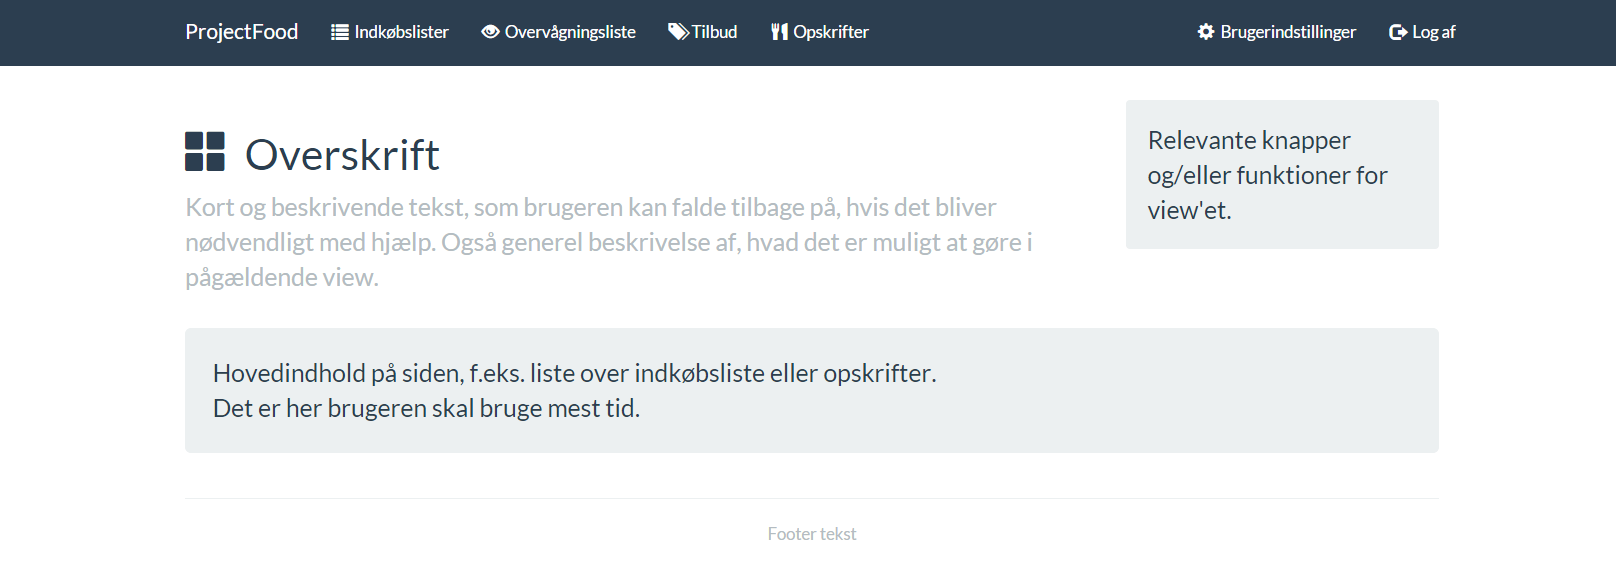
\includegraphics[trim=3.5cm 0cm 3cm 0cm, clip=true, width=1\textwidth]{images/Images/generelt_layout.png}
\caption{Design skabelon som beskriver den umiddelbare inddeling af views i systemet.}\label{ss:design_skabelon}
\end{figure}
Skabelonen er bygget op med tre hovedgrupper, foruden navigerings-baren og footeren. En gruppe til ikon(glyphicon), overskrift og forklarende hjælpetekst, en anden gruppe til knapper og relevante funktioner (det kunne f.eks. være en ``Opret indkøbsliste''-knap), og en tredje gruppe til selve hovedindholdet.
I HTML syntaks vil \myref{ss:design_skabelon}, se således ud:
\begin{lstlisting}[language=HTML, caption=HTML-kode med de tre hoved grupper, label=html:design_skabelon]
<div class="page-header nopadding-xs">
    <div class="container-fluid nopadding">
        <div class="col-md-9 col-xs-12 nopadding">
            <!--- Første gruppe --->
            <h1><span class="glyphicon glyphicon-th-large"></span>&nbsp;&nbsp;Overskrift</h1>
            <p class="hidden-xs lead text-muted nopadding">
                Kort og beskrivende tekst, som brugeren kan falde tilbage på, hvis det bliver nødvendligt med hjælp.
                Også generel beskrivelse af, hvad det er muligt at gøre i pågældende view.
            </p>
            <!--- Første gruppe slut --->
        </div>
        <div class="col-md-3 col-xs-12 nopadding">
            <!--- Anden gruppe --->            
            <div class="well lead">
                Relevante knapper og/eller funktioner for view'et.
            </div>
            <!--- Anden gruppe slut --->
        </div>
    </div>
</div>
<div class="container-fluid nopadding">
    <!--- Tredje gruppe --->
    <div class="well well-lg lead">
        Hovedindhold på siden, f.eks. liste over indkøbsliste eller opskrifter.<br />
        Det er her brugeren skal bruge mest tid.
    </div>
    <!--- Tredje gruppe slut --->
</div>
\end{lstlisting}

I denne kode anvendes Bootstrap klasser. 
Gitter-systemet som Bootstrap stiller til rådighed bruges, for at få at opnå det ønsket layout og på samme tid tilpasses den mobil-platform.
Vi har udviklet vores egne CSS-klasser som f.eks. \texttt{nopadding}, for at kunne tilpasse layoutet yderligere. 
Med denne blanding af Bootstrap og vores eget CSS, kan vi tilpasse systemet præcis som vi vil. 
En af de andre funktioner, vi benytter fra Bootstrap, er \textit{glyphicons}, som øger hjemmesidens consistency og affordance.
Disse \textit{glyphicons} bruges bl.a. i overskrifter, og i navigerings-baren.

\textbf{Mobil tilpasning}\hfill\\
Det meste af vores tilpasning til mobil-platformen, klares af bootstaps responsive design, som er opnået ved at definere forskellige atributter for forskellige skærm størrelser.
Derudover benytter vi os af CSS-klasser, fra Bootstrap, som kan skjule og/eller vise ting ved netop forskellige skærm størrelser.
Vi vælger derved at begrænse systemets funktionalitet for brugeren, når de tilgår det via en mobil-platform. De funktioner, som vi skjuler for brugeren, er:

\begin{description}
\item[Oprettelse, redigering og kloning af opskrifter]\hfill\\
Grunden til, at vi har valgt at begrænse brugeren for denne funktionalitet på mobil-platformen, er at denne platform ikke er tænkt som et sted, hvor man skal foretage forholdvis kompliceret data oprettelse eller ændring.
Samtidigt fokuserer vi opskrifts komponenten omkring den relevate kontekst, når mobil-platforment benyttes, som er inspirationssøgning eller madlavning - i disse kontekster er det kun nødvendigt at kunne finde opskrifter og følge dem.
\item[Muligheden for at ændre kodeord]\hfill\\
Dette er ikke noget brugeren vil gøre ofte, og derfor har vi valgt, at ekskludere denne funktion fra mobil-platformen.
\end{description}

Når vi vælger at skjule funktionalitet for brugeren, er det udelukkende for at give brugeren en bedre oplevelse med brugen af hjemmesiden på mobil-platformen.
Vi påfører \textit{constraints} og på den måde, forhindres brugeren i, at tilgå steder der ikke egner sig til mobil-platformen.
Med fordel kunne man inkoorporere alle funktioner vha. \textit{overflow menuer} bl.a. kendt fra Google's tjenester, hvor tre prikker indikerer at yderligere funktionalitet er tilgængelig. \cite{actionbar}
På denne måde vil brugere, der udelukkende benytter sig at smartphones eller lign. også være i stand til at kunne udnytte alle hjemmesidens funktionaliteter.

\begin{wrapfigure}{o}{0.42\textwidth}
\vspace{-30pt}
\begin{center}
\textit{Desktop}
\frame{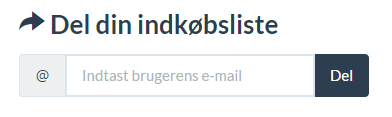
\includegraphics[width=0.4\textwidth]{images/Images/share_desktop.png}}\\
\vspace{10pt}
\textit{Mobil (efter tryk på knap)}
\frame{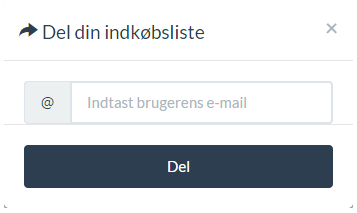
\includegraphics[width=0.4\textwidth]{images/Images/share_modal.png}}
\end{center}
\vspace{-10pt}
\caption{Her ses henholdsvis desktop- og mobil-udgaven af \textit{del-funktionen}}\label{ss:share_diffs}
\vspace{-30pt}
\end{wrapfigure}
Nogle steder har vi istedet for at gemme en funktionalitet væk, erstattet f.eks. en tekstboks med en knap, der så generere et vindue med de elementer der skal til for at udføre handlingen. 
Et eksempel på dette ses, når en bruger vil dele sin indkøbsliste med andre brugere.
På en computer vil man blive præsenteret for en tekstboks, med dertilhørende knap, mens mobil-udgaven viser brugeren en knap med titlen \textit{Del}, som generere et pop-up over selve siden, når de trykker på den (se \myref{ss:share_diffs} ).

\textbf{Respons til brugerinput}\hfill\\
For at brugeren oplever systemet som \textit{levende}, har vi implementeret forskellige former for respons og visuel feedback.
Dette gøres gennem jQuery og Bootstrap klasser.
Med Javascript og jQuery, kan man tilføje og fjerne klasser fra HTML tags, samt genere HTML kode uden at genindlæse siden - på den måde virker det for brugeren som om, at siden er \textit{levende}.
Vi har derudover valgt at benytte os af et javascript framework, kaldet \class{snackbar.js}, der tillader os, at præsentere brugeren for en snackbar.
En snackbar er, i dette tilfælde, en lille besked der popper op i nederste venstre hjørne af skærmen; snackbaren kan indeholde en hvilken som helst besked, og vi kan endvidere vise glyphicons deri.
Nogle eksempler på dette er:
\begin{description}
\item[Tilføje varer til indkøbsliste, fra tilbud side eller opskrift]\hfill\\
Ud for hvert tilbud, på tilbuds siden, og ingredienser på opskrifter, er det muligt for brugeren at trykke på en blå knap, der er præsenteret med et plus (\textbf{+}). 
Når varen bliver tilføjet, vil brugeren opleve, at knappen skifter farve til grøn, og plusset bliver til et flueben.
Derudover vil en snackbar komme til syne, med en besked om, at det er lykkedes at tilføje varen til den valgte indkøbsliste.
(Se \myref{code:user_feedback} funktion nr. 1)
\item[Ændre hvilke butikker man ønsker at se tilbud fra]\hfill\\
Under brugerindstillinger, er der ud for alle butikker vist en checkboks, som systemet har fundet tilbud fra.
Som udgangspunkt er alle butikker tilvalgt, hvilket er vist med et flueben i checkboksen.
Når brugeren så vælger at fjerne en butik, vil fluebenet forsvinde, og teksten bliver overstreget og faded ud.
Vi informerer også brugeren om, at indstillingen er gemt, med en snackbar.
(Variation af funktion nr. 1 på \myref{code:user_feedback})
\item[Dele indkøbsliste med andre brugere]\hfill\\
Hvis brugeren forsøger at dele sin indkøbsliste med en anden bruger, præsenterer vi resultatet af handlingen igennem en snackbar.
På denne måde kan brugeren se, om det er lykkedes eller om den indtastede email ikke findes.
(Udvidelse af funktion nr. 2 på \myref{code:user_feedback})
\end{description}

\begin{lstlisting}[language=JavaScript,caption={Javascript funktioner, der giver bruger feedback},label=code:user_feedback]
function ChangeToCheckRecipe(json) {
    var recipeButton = '#AddItem_' + json.itemID;
    $(recipeButton)
        .removeClass('btn-info')
        .addClass('btn-success')
        .blur();
    $(recipeButton + ' span')
        .removeClass('glyphicon-plus')
        .addClass('glyphicon-ok');
    MakeSnackbar("Vare tilføjet til " + json.shoppingListTitle, "glyphicon-ok", "toast", "1500");
};

//Generate snackbar and show on screen. text, glyphicon, style and timeout is optional.
function MakeSnackbar(text, glyphicon, style, timeout) {
    $('#snackbar-container').children().each(function () {
        $(this).snackbar('hide');
    });
    var options;
    if (isset(glyphicon)) {
        var glyphiconContainer = $('<div>');
        var span = $('<span>').addClass('glyphicon').addClass(glyphicon);
        glyphiconContainer.append(span);
        options = {
            content: glyphiconContainer.html() + "&nbsp;&nbsp;" + ((isset(text)) ? text : " "),
            style: (isset(style)) ? style : "snackbar",
            timeout: (isset(timeout)) ? timeout : 2500
        };
    } else {
        options = {
            content: (isset(text)) ? text : " ",
            style: (isset(style)) ? style : "snackbar",
            timeout: (isset(timeout)) ? timeout : 2500
        };
    }
    $.snackbar(options);
};
\end{lstlisting}

\subsection{Konklusion}
Med vores design skabelon og brugen af \textit{glyphicons}, forøger vi niveauet af \textbf{learnability} markant, og brugeren får i sidste ende lettere ved at bruge hjemmesiden.
For at opfylde kravet om \textbf{effectiveness}, benytter vi os af constraints, bl.a. begrænset funktionaliteterne i forskellige kontekster.
\textbf{Ease of use} opnås ved, at systemet giver brugeren feedback, når der foretages forskellige handlinger.
Her er muligheden for at lave \textit{snackbars} en essentiel del.
Brugen af vores design skabelon, samt navigerings-baren, hjælper også med til at overholde Getalts love om perception, i form af gruppering.
Guidelines omkring mobile-platforme, overholder vi bl.a. igennem overvejelser ift. konteksten i udviklingen af vores views.
Eftersom vi ikke har valgt at udvikle en dedikeret app, til smartphones, hjælper det også meget på brugeroplevelsen, at vi kan præsentere den mobile-udgave uden url-baren der normalt optræder i browseren.

